
\chapter{实验}\label{chapter_experiment}
为了验证自动化检测工具的可行性、正确性,在本章中将设计实验进行验证。

首先将会设计仿真测试,在仿真测试中,会设计轻量级的、最简单的仿真应用,以检验自动检测工具是否能够正确检测出内存泄漏的组件,同时不出现误检的行为。

接下来为了评价在安卓10上服务和广播接收器的内存泄漏情况,将会从安卓应用市场中下载真实的应用,使用本文所述的工具进行测试,得出结论。
\section{仿真测试}

\subsection{仿真应用}

仿真应用应同时具有两个\textbf{公开服务}以及两个\textbf{清单声明的广播接收器}。其中每个控件之一需要人为制造内存泄漏(称为\textbf{LeakedService(Listing.\redbf{\ref{code:LeakedService}})}与\textbf{LeakedReceiver(Listing.\redbf{\ref{code:LeakedReceiver}})}),另一个则需要确保不存在内存泄漏(称为\textbf{NormalService(Listing.\redbf{\ref{code:Normal}})}与\textbf{NormalReceiver(Listing.\redbf{\ref{code:Normal}})})。
在对仿真应用进行测试时,预期的实验结果为:能够检测到\textbf{LeakedService}和\textbf{LeakedReceiver}的泄露实例,以证明该工具可以发现内存泄漏问题;而检测不到\textbf{NormalService}和\textbf{NormalReceiver}的泄露实例,以证明该工具不会将正常的组件误检。


\begin{listing}[htbp]
	\centering
	\caption{\textbf{LeakedService}主体代码}
	\begin{minted}[encoding=utf8,
	frame=single,
	framesep = 1em,
	numbers=left, 
	breaklines=true, 
	tabsize=4,
	xleftmargin=2em,xrightmargin=2em,
	fontsize=\footnotesize]{java}
public class LeakedService extends Service {
	private static final String TAG = "LeakedService";
	@Override
	public void onCreate() {
		super.onCreate();
		new Timer().scheduleAtFixedRate(new TimerTask() {
			@Override
			public void run() {
				Log.i(TAG,LeakService.this.getPackageName() + ".LeakService running ");
			}
		},1000L,3000L);
	}
}	
	\end{minted}
	\label{code:LeakedService}
\end{listing}

\begin{listing}[htbp]
	\centering
	\caption{\textbf{LeakedReceiver}主体代码}
	\begin{minted}[encoding=utf8,
	frame=single,
	framesep = 1em,
	numbers=left, 
	breaklines=true, 
	tabsize=4,
	xleftmargin=2em,xrightmargin=2em,
	fontsize=\footnotesize]{java}
public class LeakedReceiver extends BroadcastReceiver {
	private static final String TAG = "LeakedReceiver";
	private final Random random = new Random();
	@Override
	public void onReceive(Context context, Intent intent) {
		new Timer().scheduleAtFixedRate(new TimerTask() {
			@Override
			public void run() {
				Log.i(TAG,LeakReceiver.this.random.nextInt() + ".LeakReceiver running ");
			}
		},1000L,3000L);
	}
}
	\end{minted}
	\label{code:LeakedReceiver}
\end{listing}

\begin{listing}[htbp]
	\centering
	\caption{\textbf{NormalReceiver}与\textbf{NormalService}主体代码}
	\begin{minted}[encoding=utf8,
	frame=single,
	framesep = 1em,
	numbers=left, 
	breaklines=true, 
	tabsize=4,
	xleftmargin=2em,xrightmargin=2em,
	fontsize=\footnotesize]{java}
public class NormalReceiver extends BroadcastReceiver {
	private static final String TAG = "NormalReceiver";
	private final Random random = new Random();
	@Override
	public void onReceive(Context context, Intent intent) {
		Log.i(TAG,NormalReceiver.this.random.nextInt() + ".NormalReceiver running ");
		}
	}
}

public class NormalService extends Service{
	private static final String TAG = "NormalService";
		@Override
	public void onReceive(Context context, Intent intent) {
		Log.i(TAG,NormalService.this.getPackageName() + ".LeakService running ");
	}
}
	\end{minted}
	\label{code:Normal}
\end{listing}
\subsection{实验结果}
实验结果(见\textbf{图.}\redbf{\ref{fig:result of mock receiver}}及\textbf{图.}\redbf{\ref{fig:result of mock service}})能正确检测到\textbf{LeakedService}和\textbf{LeakedReceiver}的内存泄漏实例,而没有误检\textbf{NormalService}以及\textbf{NormalReceiver},证明检测工具实际有效。

\begin{figure}[htbp]
	\centering
	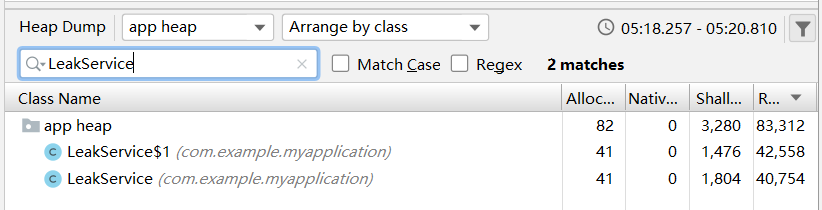
\includegraphics[width=0.9\textwidth]{service_leak_result.png} % requires the graphicx package
	\caption{检测到\textbf{LeakedService}内存泄漏实例}
	\label{fig:result of mock service}
\end{figure}
\begin{figure}[htbp]
\centering
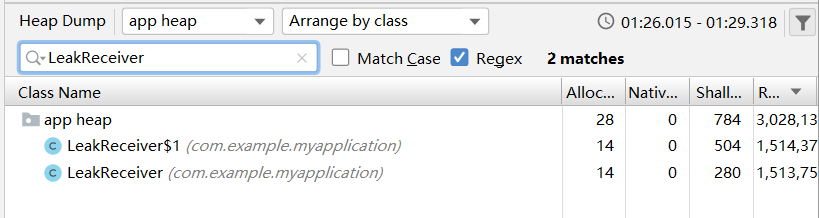
\includegraphics[width=0.9\textwidth]{receiver_leak_result.png} % requires the graphicx package
\caption{检测到\textbf{LeakedReceiver}内存泄漏实例}
\label{fig:result of mock receiver}
\end{figure}

\newpage
\section{真实测试}


本文选取了\textbf{AppChina 应用市场}\cite{appchina}作为测试应用的来源,在其中的\textbf{视频},\textbf{游戏},\textbf{工具}三个类别中,选取了每个分类中当月下载量最高的若干应用进行测试,共计\textbf{22}个。对这\textbf{22}个应用的测试结果详见\textbf{\redbf{\ref{now-result}}小节}:

\subsection{实验结果}\label{now-result}
\textbf{表现正常 12(54.5\%) }这些应用的组件表现正常,并没有出现内存泄露问题。

\textbf{内存泄漏 3(13.6\%) }这些应用包含了存在内存泄漏问题的组件,并成功被检测工具检测到。

\textbf{应用崩溃 7(31.8\%) }这些应用在测试时抛出了\textbf{ANR(Application Not Response)}异常,导致应用崩溃,无法完成测试。

\subsection{应用崩溃主要原因分析}

\textbf{无法正常启动 } 部分应用在启动时即发生了崩溃,导致应用停止运行。这类应用崩溃的原因可能是应用的版本和模拟器系统的版本不兼容,例如使用了不再符合开发规范的接口,某些接口不再支持,或没有在\textbf{AndroidManifest.xml}中声明所需的权限(缺少\textbf{<uses-permission>}标签)等。

\textbf{在测试过程中崩溃 } 部分应用可以正常启动,但是在\textbf{主测试流程}中发生了应用崩溃问题。这类应用崩溃的原因可能是因为应用的组件启动流程存在问题,比如:进行了风险操作,进行了线程不安全操作,没有对启动环境进行检查等;也可能是由于应用的组件确实存在\textbf{内存泄漏}问题,而且泄露表现的十分严重,触发了安卓系统的安全限制,导致安卓系统介入将应用停止运行。

\textbf{空指针异常 } 部分应用的组件在启动时会抛出\textbf{NullPointerException},该异常表示,在组件的启动过程中,对未实例化的对象进行了读写操作。这类问题大多数是因为组件的开发人员的疏忽,导致的程序缺陷。可能的成因有组件之间使用了共享资源,但是并没有进行专门管理,也有可能是因为这类组件的启动严格遵循\textbf{状态自动机},但是测试时无法得知组件启动需要满足的前置条件,导致运行出错。

\section{结果分析}

本小节会将本文的测试结果(见\ref{now-result})计算指标来进行分析。

\subsection{数据分析}
\begin{table}[htb]\footnotesize
	\centering
	\caption{实验数据及指标}
	\vspace{2mm}
	% l - left, r - right, c - center. | means one vertical line 这里声明的是表格单元中的内容如何对齐
	\begin{tabular}{lcccc}
		\toprule
		&\textbf{表现正常}&\textbf{内存泄漏}&\textbf{运行异常}&\textbf{泄露正常比}\\
		\midrule
		\textbf{指标}&54.5\%&13.6\%&31.8\%&0.250\\
		\bottomrule
	\end{tabular}
	\label{table:compare}
\end{table}

实验数据的对比表明:
\begin{itemize}
	\item 存在内存泄漏的应用比例为\textbf{13.6\%},说明组件内存泄漏现象较为普遍。
	\item 运行异常的应用比例为\textbf{31.8\%},说明安卓组件碎片化问题比较严重,兼容性问题相对于内存泄漏问题更为明显。兼容性问题具体原因有:安卓版本升级后,系统权限的收紧,导致应用无法像先前版本一样正常获取响应权限;组件的开发规范变更,导致原有代码抛出异常,导致应用崩溃等。
	\item 泄露正常比(检测到内存泄漏问题的应用数量与表现正常的应用数量之比)为\textbf{0.250},这项指标相较于\textbf{内存泄漏应用的比例}更有实际意义,它说明了在\textbf{经过成熟测试的稳定可用的应用}中,组件的内存泄漏问题依然较为普遍,这要求开发者在进行不可见组件开发的时候,需要投入更多的精力进行测试和调试,以确保这些组件中不会出现程序缺陷。
\end{itemize}

\subsection{实验数据局限性}

由于实验设备和实验环境的限制(参考\textbf{表.}\redbf{\ref{table:pc-compare}}),本文只能使用效率较慢的方式对少量小规模的应用进行串行的测试(参考\textbf{表.}\redbf{\ref{table:method-compare}})。因此实验结果具有较大的局限性。
\newline

\begin{table}[htb]\footnotesize
	\centering
	\caption{工作站配置}
	\vspace{2mm}
	% l - left, r - right, c - center. | means one vertical line 这里声明的是表格单元中的内容如何对齐
	\begin{tabular}{lcccc}
		\toprule
		&\textbf{操作系统}&\textbf{内存容量}&\textbf{处理器型号}&\textbf{模拟器系统版本}\\
		\midrule
		\textbf{测试配置}&Windows 10&8 GB&Intel(R) Core(TM) i7-8565U&Android 10\\
		\bottomrule
	\end{tabular}
	\label{table:pc-compare}
\end{table}

\begin{table}[htb]\footnotesize
	\centering
	\caption{测试方法}
	\vspace{2mm}
	% l - left, r - right, c - center. | means one vertical line 这里声明的是表格单元中的内容如何对齐
	\begin{tabular}{lcccc}
		\toprule
		&\textbf{并发能力}&\textbf{模拟器内存}&\textbf{模拟器SD卡容量}&\textbf{测试强度}\\
		\midrule
		\textbf{测试方法}&单线程&2 GB&512 MB&每个应用测试2次\\
		\bottomrule
	\end{tabular}
	\label{table:method-compare}
\end{table}

\section{小结}
在本章中,设计了仿真测试实验,以及真实测试实验。前者验证了自动化检测工具的正确性和可行性,而后者研究了安卓10中,应用的组件内存泄漏的发生几率,一定程度上验证了安卓组件开发碎片化的问题,同时证明安卓不可见控件内存泄漏的问题依然广泛存在。